\documentclass[a4paper,12pt, oneside]{book}

% \usepackage{fullpage}
\usepackage[italian]{babel}
\usepackage[utf8]{inputenc}
\usepackage{amssymb}
\usepackage{amsthm}
\usepackage{graphics}
\usepackage{amsfonts}
\usepackage{listings}
\usepackage{amsmath}
\usepackage{amstext}
\usepackage{engrec}
\usepackage{rotating}
\usepackage[safe,extra]{tipa}
%\usepackage{showkeys}
\usepackage{multirow}
\usepackage{hyperref}
\usepackage{mathtools}
\usepackage{microtype}
\usepackage{enumerate}
\usepackage{braket}
\usepackage{marginnote}
\usepackage{ulem}
\usepackage{bm}
\usepackage{pgfplots}
\usepackage{cancel}
\usepackage{polynom}
\usepackage{booktabs}
\usepackage{enumitem}
\usepackage{framed}
\usepackage{algorithm}
\usepackage{algpseudocode}
\usepackage{pdfpages}
\usepackage{pgfplots}
\usepackage[cache=false]{minted}

\usepackage[usenames,dvipsnames]{pstricks}
\usepackage{epsfig}
\usepackage{pst-grad} % For gradients
\usepackage{pst-plot} % For axes
\usepackage[space]{grffile} % For spaces in paths
\usepackage{etoolbox} % For spaces in paths
\makeatletter % For spaces in paths
\patchcmd\Gread@eps{\@inputcheck#1 }{\@inputcheck"#1"\relax}{}{}
\makeatother

\usepackage{tikz}\usetikzlibrary{er}\tikzset{multi
  attribute /.style={attribute ,double  distance =1.5pt}}\tikzset{derived
  attribute /.style={attribute ,dashed}}\tikzset{total /.style={double
    distance =1.5pt}}\tikzset{every  entity /.style={draw=orange ,
    fill=orange!20}}\tikzset{every  attribute /.style={draw=MediumPurple1,
    fill=MediumPurple1!20}}\tikzset{every
  relationship /.style={draw=Chartreuse2, fill=Chartreuse2!20}}
\newcommand{\key}[1]{\underline{#1}}

\usepackage{fancyhdr}
\pagestyle{fancy}
\fancyhead[LE,RO]{\slshape \rightmark}
\fancyhead[LO,RE]{\slshape \leftmark}
\fancyfoot[C]{\thepage}
\usepackage{tikz}
\usetikzlibrary{automata,positioning}


\title{Assignment 3, Bioinformatica}
\author{Davide Cozzi, 829827}
\date{}

\pgfplotsset{compat=1.13}
\begin{document}
\maketitle

\definecolor{shadecolor}{gray}{0.70}
\setlist{leftmargin = 2cm}
\newtheorem{teorema}{Teorema}
\newtheorem{definizione}{Definizione}
\newtheorem{esempio}{Esempio}
\newtheorem{corollario}{Corollario}
\newtheorem{lemma}{Lemma}
\newtheorem{osservazione}{Osservazione}
\newtheorem{nota}{Nota}
\newtheorem{esercizio}{Esercizio}

\renewcommand{\chaptermark}[1]{%
  \markboth{\chaptername
    \ \thechapter.\ #1}{}}
\renewcommand{\sectionmark}[1]{\markright{\thesection.\ #1}}
\tableofcontents
\chapter{Esercizio}
\section{Svolgimento}
Per semplicità si assume che la sequenza in input è data su alfabeto
$\Sigma=\{A,C,G,T\}$.\\
Viene data in input la sequenza:
\[S=ACCGCGCTCGCGTACCTT\]
con l'obiettivo di dare una rappresentazione succinta del suo \textbf{grafo di
  De Bruijn} dato $k=5$ (in modo da avere nodi di lunghezza pari a $4$ come da
specifica): 
\begin{figure}[H]
  \centering
  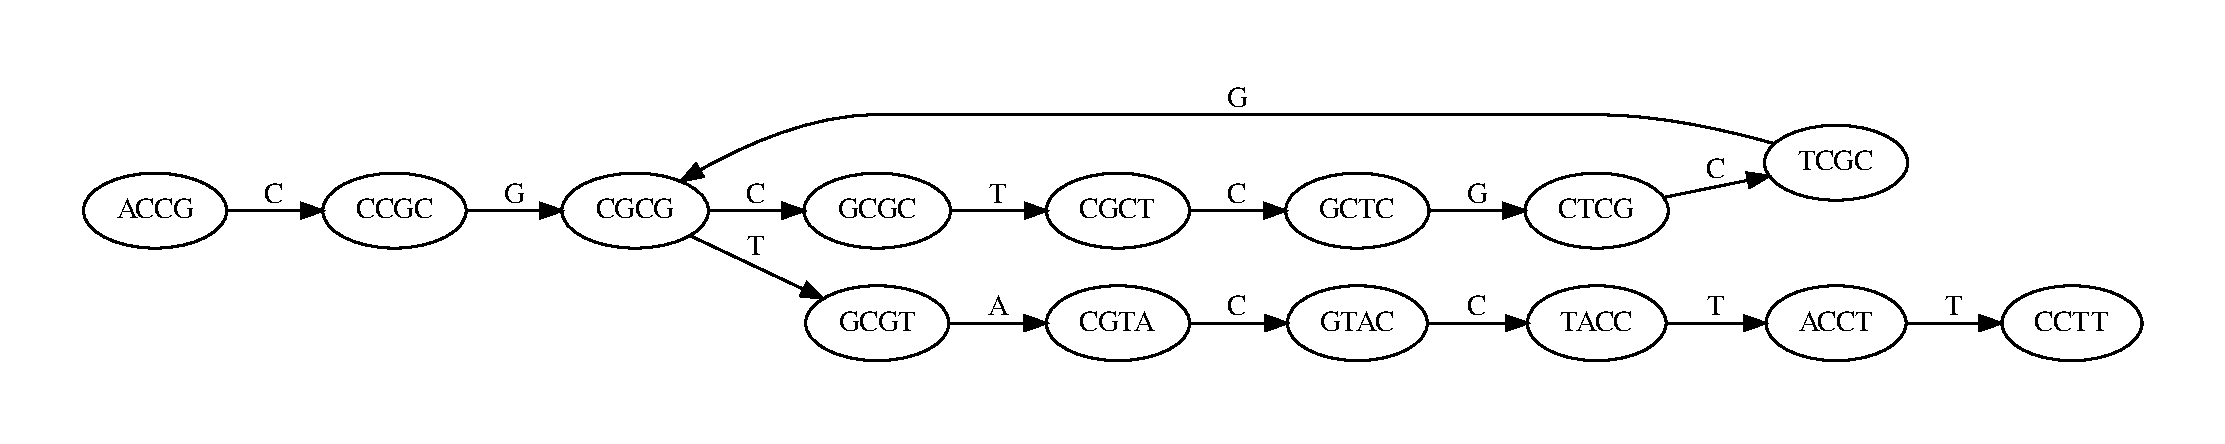
\includegraphics[width = \textwidth]{img/assign3nd.pdf}
  \caption{Grafo di De Bruijn della sequenza $S$.}
\end{figure}
Per poter avere una rappresentazione corretta del \textbf{grafo di De Bruijn
  succinto} bisogna in primis procedere con l'apposizione di una quantità di
$\$$ pari a $k-1$ in modo da ottenere un nodo composto da soli $\$$ nel nostro
grafo e permettere la corretta visita dello stesso (come si vedrà dopo a causa
dell'array $F$). Avendo $k=5$ si ottiene quindi:
\[S=\$\$\$\$ACCGCGCTCGCGTACCTT\]
\newpage
Si procede quindi alla rappresentazione succinta del grafo tramite:
\begin{itemize}
  \item l'array $last$, per rappresentare la presenza multipli archi in uscita
  da un nodo 
  \item l'array $W$, per rappresentare le etichette degli archi. Si segnala che
  si possono avere etichette marcate come
  \textit{negative}, tramite il simbolo ``-'', che segnalano eventuali archi con
  la stessa etichetta che puntano allo stesso nodo partendo da due nodi
  diversi. Quest'ultimo dettaglio è comunque solo interno alla rappresentazione,
  non aspettandoci query, nello studio del grafo, con simboli già segnati
  negativi
  \item l'array $F$, per rappresentare in modo compatto l'array che sarebbe
  formato degli ultimi caratteri delle etichette dei nodi, ordinate in ordine
  lessicografico ``da destra''. Tale array $F$ lo possiamo memorizzare in modo
  compatto, in ``forma'' analoga alla
  funzione $C$ di un ipotetico \textbf{FM-index} costruito sull'array degli
  ultimi caratteri delle etichette dei nodi, grazie al fatto che i simboli sono
  ordinati lessicograficamente. Diventa quindi fondamentale avere
  il primo nodo del grafo con etichetta di soli \$, in modo da avere almeno un
  \$ nell'array degli ultimi simboli e poter costruire, nonché poi usare,
  correttamente l'array $F$ 
\end{itemize}
Si ottiene quindi rappresentazione del grafo come da tabella \ref{tab:dbg}
(dove, dei valori in tabella, solo $last$ e $W$ sono in memoria mentre le altre
informazioni sono mostrate per semplicità nello studio dell'esercizio).
\begin{table}
  \centering
  \begin{tabular}{c|c||c|c||c|c}
    edge index & node index & \textbf{\textit{last}} & \textbf{\textit{W}}
    & label & last char label\\
    \hline
    0 & 0 & 1 & A & \$\$\$\$ & \$ \\
    1 & 1 & 1 & C & \$\$\$A & A \\
    2 & 2 & 1 & C & CGTA & A \\
    3 & 3 & 1 & C & \$\$AC & C \\
    4 & 4 & 1 & C & GTAC & C \\
    5 & 5 & 1 & G & \$ACC & C \\
    6 & 6 & 1 & T & TACC & C \\
    7 & 7 & 1 & G & CCGC & C \\
    8 & 8 & 1 & T & GCGC & C \\
    9 & 9 & 1 & G- & TCGC & C \\
    10 & 10 & 1 & G & GCTC & C \\
    11 & 11 & 1 & C & ACCG & G \\
    12 & 12 & 0 & C & CGCG & G \\
    13 & 12 & 1 & T & CGCG & G \\
    14 & 13 & 1 & C & CTCG & G \\
    15 & 14 & 1 & T & ACCT & T \\
    16 & 15 & 1 & C & CGCT & T \\
    17 & 16 & 1 & A & GCGT & T \\
    18 & 17 & 1 & \$ & CCTT & T \\
  \end{tabular}
  \caption{Tabella con le informazioni in memoria, $last$ e $W$, per l'esercizio
  con l'aggiunta di alcune informazioni extra. Come informazioni aggiuntive
  troviamo in primis gli indici dei nodi e gli indici degli archi, che verranno
  spesso usati nell'esercizio. Troviamo poi le label dei nodi e l'array degli
  ultimi simboli delle label dei nodi, ordinate lessicograficamente a partire da
  destra. Quest'ultima colonna viene memorizzata in modo compatto nell'array
  $F$.} 
  \label{tab:dbg}
\end{table}
\\
\noindent
Come detto in memoria si ha anche l'array $F$, una rappresentazione compatta di
quello che nella tabella è indicato con \textit{last char label}. L'array $F$
prodotto per l'esercizio è quindi:
\begin{gather*}
  F[\$] = 0\\
  F[A] = 1\\
  F[C] = 3\\
  F[G] = 11\\
  F[T] = 15
\end{gather*}
Una rappresentazione grafica del grafo è visibile in figura \ref{fig:dbg}.
\begin{figure}
  \centering
  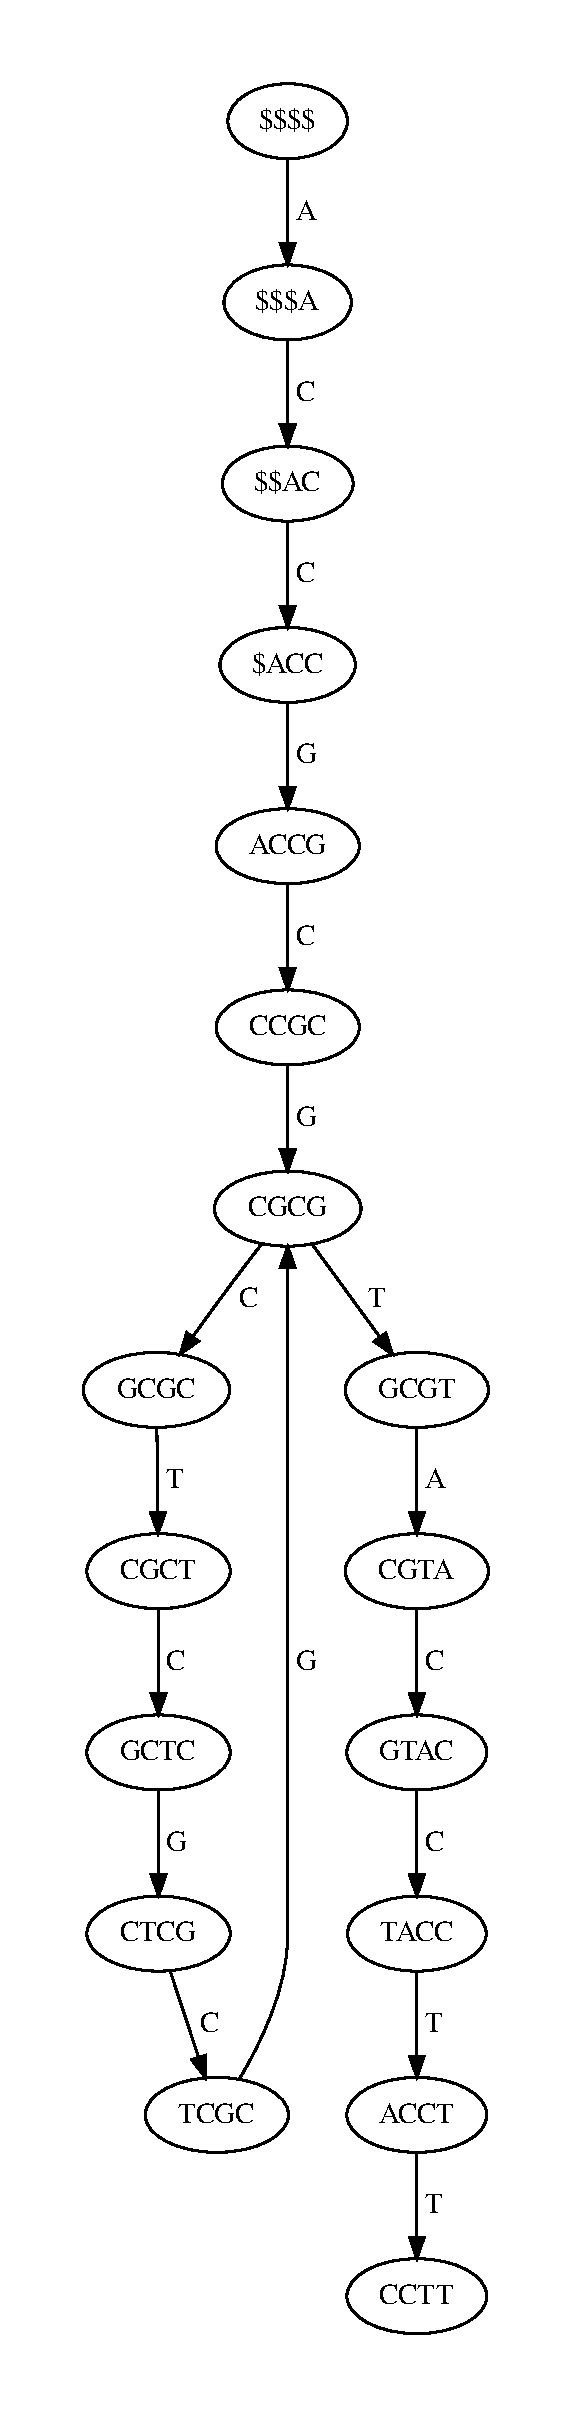
\includegraphics[scale = 0.47]{img/assign3v.pdf}
  \caption{Rappresentazione grafica, comoda per visualizzare quanto trattato,
    del grafo di De Bruijn della 
    sequenza $S$, con i dovuti \$ a sinistra e relativi nodi nel grafo docuti
    alla rappresentazione succinta del grafo stesso.}
  \label{fig:dbg}
\end{figure}
\\
\noindent
Si cerca quindi di capire, dato un nodo $v$, come passare ad un nodo $v'$,
tramite uno degli archi uscenti da $v$, etichettato con $l$. Avendo quindi $v$ e
$v'$ rappresentati con un indice, avendo che la numerazione degli stessi è
indicizzata a partire da 0, si cerca di costruire una funzione
$v'=outgoing(v,l)$ che, preso in input un nodo $v$, in forma di indice, e
un'etichetta $l$, calcola $v'$, qualora esista, che è il nodo, sempre in forma
di indice, in cui si arriva partendo da $v$ tramite un arco etichettato con
$l$. Qualora tale nodo $v'$ non esista si restituisce $-1$. Si ha quindi:
\[outgoing(v,l)=
  \begin{cases}
    v' &\mbox{se tale nodo $v'$ esiste}\\
    -1 &\mbox{altrimenti}
  \end{cases}
\]
Il calcolo di tale funzione, nonché in generale l'intero studio dei
\textbf{grafi di De Bruijn succinti}, si basa su due funzioni che bisogna
definire: 
\textbf{rank} e \textbf{select}.
\begin{definizione}
  Si definisce la funzione $\mathbf{rank_s(x)}$ come la funzione che permette di
  calcolare, in un vettore $V$ di $n$ elementi, il numero di occorrenze
  di un simbolo $s$ tra la posizione 0 e una posizione $x$ passata come
  argomento alla funzione.
\end{definizione}
\begin{definizione}
  Si definisce la funzione $\mathbf{select_s(x)}$ come la funzione che permette
  di calcolare, in un vettore $V$ di $n$ elementi, l'indice dell'$x$-esimo
  simbolo uguale a $s$.
\end{definizione}
\noindent
\textit{Nel nostro caso parlando di $rank_s$ e $select_s$, per un simbolo $s$,
  si assume che si lavora sempre sull'array $W$ mentre con $rank_1$ e $select_1$
  si assume di lavorare sull'array $last$}.\\
\textit{Per comodità, inoltre, si suppone di essere in grado di effettuare
  queste due operazioni anche su un simbolo $s$ marcato come negativo senza
  ulteriori specifiche, come se fosse un simbolo come un altro, ovviamente
  diverso dal suo corrispondente non negato. A livello di codice, nella bozza
  implementata, il discorso in merito sarà ``meno ottimizzato''}.\\
Per poter discutere della funzione $outgoing(v,l)$ abbiamo bisogno di un'altra
operazione fondamentale per ``navigare'' un \textbf{grafo di De Bruijn}
memorizzato in forma succinta, la funzione $forward(e)$.
\begin{definizione}
  Si definisce la funzione $\mathbf{forward(e)}$ come la funzione che
  restituisce l'indice dell'ultimo arco, che quindi presenta $1$ nell'array
  $last$, del nodo a cui si punta tramite l'arco $e$. Qualora tale nodo non
  esista, non potendo quindi restituire l'indice del suo ultimo arco, si
  restituisce $-1$.  
\end{definizione}
\noindent
Vediamo quindi indicativamente il funzionamento di tale funzione, notando come
il ragionamento può essere pensato in modo a tratti simile, ma, come si vedrà,
non in modo identico, a quanto si farebbe con 
LF-mapping tra l'array $W$ e l'array chiamato $last$ $char$ $label$, in tabella
\ref{tab:dbg}: 
\begin{itemize}
  \item si estrae in primis il simbolo che etichetta l'arco $e$, banalmente
  usando l'array $W$:
  \[s \gets W[e]\]
  Se tale simbolo è uguale a $\$$ si restiuisce $-1$ e si interrompe
  l'esecuzione in quanto sappiamo che non possiamo avere archi etichettati con
  $\$$, per costruzione, e che nell'array $W$ essi rappresentano appunto un arco
  fittizio (rappresentando un arco ipotetico, non avendo quindi mancanza di
  informazione in $W$, uscente da un nodo ``pozzo'')
  \item si calcola quindi, sull'array $W$, quanti sono i simboli $s$ presenti
  fino all'indice $e$, in modo da ottenere un ordine relativo del carattere $s$ su
  $W$. Per farlo basta usare la funzione $rank_s$: 
  \[rindex \gets rank_s(e)\]
  \item si cerca l'indice della prima occorrenza di $s$ su $last$ $char$
  $label$, tramite l'array $F$:
  \[focc \gets F[s]\]
  \item bisogna poi capire quanti nodi ci siano prima dei nodi "candidati",
  ovvero quei nodi che hanno etichette con ultimo simbolo pari a $s$. Per farlo
  si verificano quanti $1$ ci sono sull'array $last$ prima della prima
  occorrenza di un nodo "candidato", usando la funzione $rank_1$:
  \[nprevs \gets rank_1(focc-1)\]
  \item infine si può ottenere l'indice dell'ultimo arco uscente dal nodo a cui
  si punta tramite l'arco $e$. Sapendo quanti simboli $s$ precedono il simbolo
  voluto su $W$ (che è stato definito sopra come $rindex$) e quanti nodi ho
  prima dei candidati possibili (che è stato definito sopra come $nprevs$) si
  può usare la funzione $select$ sull'array $last$:  
  \[e' \gets select_1(rindex + nprevs)\]
  e restituire $e'$.
\end{itemize}
\noindent
Un esempio di pseudocodice per la funzione $forward(e)$ è indicato
nell'algoritmo \ref{algo:for}.\\ 
Si è notato come in pratica si è fatto qualcosa di analogo all'LF-mapping ma
tenendo traccia di eventuali nodi con più archi uscenti. Le difficoltà di usare
direttamente LF-mapping vengono elencati alla fine dell'esercizio.
\begin{algorithm}
  \large
  \begin{algorithmic}
    \Function{forward}{$e$}
    \State $s\gets W[e]$
    \If{$s==\,'\$'$}
    \State \textbf{return} $-1$
    \EndIf
    \State $rindex \gets rank_s(e)$
    \State $focc \gets F[s]$
    \State $nprevs\gets rank_1(focc-1)$
    \State \textbf{return} $select_1(rindex+nprevs)$ 
    \EndFunction
  \end{algorithmic}
  \caption{Pseudocodice della funzione $forward$}
  \label{algo:for}
\end{algorithm}
\newpage
\begin{esempio}
  Vediamo un esempio pratico di esecuzione della funzione $forward$.\\
  Si supponga $e=13$, che corrisponde all'ultimo arco uscente dal nodo
  $CGCG$. Si ha quindi, come verificabile in tabella \ref{tab:dbg} e 
  nella rappresentazione compatta di $F$:
  \begin{itemize}
    \item $s=W[13]=T$
    \item $rindex = rank_T(13)=3$
    \item $focc = F[T]=15$
    \item $nprevs = rank_1(15-1) = rank_1(14) = 14$
    \item $e'=select_1(3+14) = select_1(17) = 17$
  \end{itemize}
  La conferma si ha, oltre che tramite figura \ref{fig:dbg}, dal fatto che,
  l'arco di indice $17$ è l'ultimo, nonché il 
  solo, relativo al nodo $GCGT$. L'arco $13$, etichettato $T$, comporta infatti:
  \[CGCG\stackrel{T}{\to}GCGT\]
  avendo conferma che la funzione è stata eseguita correttamente, avendo $GCGT$
  l'ultimo arco, nonché l'unico, indicizzato 17 in tabella \ref{tab:dbg}.\\
  In merito al discorso dell'LF-mapping è interessante notare come
  effettivamente ci si sia spostati dalla terza $T$ su $W$ alla terza $T$ su
  $last$ $char$ $label$.  
  \label{es:for}
\end{esempio}
\newpage
\noindent
Passiamo quindi allo studio effettivo della funzione $outgoing(v,l)$.\\
La funzione indicativamente esegue i seguenti passaggi:
\begin{itemize}
  \item se simbolo in input è esattamente $\$$ allora la funzione termina,
  restituendo $-1$, per lo stesso discorso fatto in merito nella spiegazione
  della funzione $forward(e)$
  \item si identifica il range di indici che indicizzano gli archi uscenti dal
  nodo $v$, avendo che tali archi saranno consecutivi nella nostra
  rappresentazione succinta.\\
  Nel dettaglio questa operazione viene effettuata tramite due operazioni di
  $select_1$ sull'array $last$, array che appunto segnala qualora un nodo abbia
  più archi uscenti:
  \[noderange(v)\gets(select_1(v)+1, select_1(v+1))=(findex, lindex)\]
  con \textit{findex} che abbrevia \textit{first index} mentre \textit{lindex}
  abbrevia \textit{last index}.
  Avendo che i due estremi di tale intervallo, appunto $select_1(v)+1$ e
  $select_1(v+1)$ segnalano, rispettivamente, il primo e l'ultimo arco uscente
  dal nodo $v$ (che si ricordi ha lo stesso \textit{node index} per ogni arco
  uscente, come visibile in tabella). Si ha quindi una tupla di indici su archi
  \item a priori non si può sapere inoltre né se esista un arco etichettato con
  $l$ che parta da $v$ e arrivi in un qualche $v'$ né tantomeno se, nella
  rappresentazione succinta, tale $l$ sia marcato come negativo nella nostra
  rappresentazione, ricordando che in input avrò sicuramente un $l$ non segnato
  negativo avendo "trasparenza" su questo aspetto. Il problema è 
  capire quale sia il corretto arco da seguire. In input alla funzione si ha
  infatti un indice di nodo, nodo che potrebbe avere più archi uscenti, coi
  rispettivi indici diversi (ma consecutivi nella rappresentazione succinta) ed
  eventuali segnature negative. Si hanno quindi tre casistiche possibili, che
  coprono il fatto che tale arco esista (segnato negativo o meno) o che non
  esista: 
  \begin{enumerate}
    \item si considera $l$ come non segnata. Tramite:
    \[nl\gets rank_l(lindex)\]
    con $lindex$ calcolato nello step precedente tramite\\ $noderange(v)$, conto
    quanti archi 
    etichettati $l$ ho fino a quell'indice. Bisogna quindi trovare l'indice
    dell'$nl$-esimo arco etichettato mediante $l$, tramite:
    \[edge \gets select_l(nl)\]
    Si è quindi ottenuto il corretto indice dell'arco uscente da $v$ ed
    etichettato con $l$.\\
    Bisogna quindi verificare che tale arco sia effettivamente nel range
    calcolato sopra, controllando che valga: 
    \[lindex\leq edge \leq findex\]
    Se esiste un arco etichetto $l$ che esce da $v$ sicuramente è in
    quel range di posizioni sull'indice degli archi.\\
    Qualora non valga si procede con la casistica 2 in quanto se fosse segnato
    negativo le funzioni rank e select lavorerebbero solo sul simbolo segnato
    negativo. \\ 
    Qualora invece valga si procede a calcolare l'indice del nodo $v'$
    effettuando in primis:
    \[edge' \gets forward(edge)\]
    per ottenere l'indice dell'ultimo dell'ultimo arco del nodo a cui si punta
    tramite l'arco $egde$. A questo punto basta usare la funzione $rank_1$ (con
    in aggiunta $-1$ per l'indicizzazione), sull'array $last$ per mappare
    l'indice dell'arco $edge'$ nel corrispettivo nodo di partenza $v'$:
    \[v'\gets rank_1(edge')-1\]
    Si interrompe quindi l'esecuzione
    \item si considera $l$ come segnata negativa, trasformando quindi $l$ in
    $l-$, e si effettuano i medesimi 
    passaggi della casistica 1. Questa
    casistica copre quei casi per cui si abbiano più nodi con archi egualmente
    etichettati che puntano ad un nodo $v'$ 
    \item se nessuno dei due casi precedenti è soddisfatto si restituisce $-1$,
    avendo che non esiste un arco etichettato con $l$ che esce dal nodo $v$. Si
    interrompe quindi l'esecuzione
  \end{enumerate}
\end{itemize}
\begin{algorithm}
  \large
  \begin{algorithmic}
    \Function{outgoing}{$v,l$}
    \If{$l==\,'\$'$}
    \State \textbf{return} $-1$
    \EndIf
    \State $(findex, lindex)\gets noderange(v)$
    \State $nl\gets rank_l(lindex)$
    \State $edge\gets select_l(nl)$
    \If{$lindex \leq edge \leq findex$}
    \State $edge'\gets forward(edge)$
    \State \textbf{return} $rank_1(edge')-1$
    \EndIf
    \State $l \gets l+ \,'-\,'$
    \State $nl\gets rank_l(lindex)$
    \State $edge\gets select_l(nl)$
    \If{$lindex \leq edge \leq findex$}
    \State $edge'\gets forward(edge)$
    \State \textbf{return} $rank_1(edge')-1$
    \EndIf
    \State \textbf{return} $-1$
    \EndFunction
  \end{algorithmic}
  \caption{Pseudocodice della funzione $outgoing$}
\end{algorithm}
\textit{Sia nella funzione $forward(e)$ che nella funzione $outgoing(v,l)$ si
  assume, per semplicità, che gli indici di archi e nodi, nonché i simboli che
  etichettano gli archi, passati come argomento alle funzioni, siano coerenti
  con la rappresentazione succinta, non avendo indici "out of bound" o simboli
  non presenti nell'alfabeto usato.} 
\newpage
\noindent
Vediamo alcuni esempi in modo da coprire le varie casistiche
\begin{esempio}
  Si prenda ad esempio il nodo 12, nell'immagine \ref{fig:dbg} etichettato con
  $CGCG$, come verificabile in tabella \ref{fig:dbg}.\\
  Tale nodo presenta come $noderange$:
  \[noderange(12)= (12,13)\]
  Avendo, infatti, complessivamente due archi uscenti dal nodo.\\
  Vediamo quindi tre ipotetici archi uscenti, uno etichettato con $T$, uno con
  $C$ e uno con $A$ (che non esiste).\\
  Iniziamo con $T$, considerata inizialmente non segnata:
  \begin{itemize}
    \item si ha in primis:
    \[nl=rank_T(13)=3\]
    \item si ha quindi:
    \[edge = select_T(3)=13\]
    \item avendo che vale $12\leq edge \leq 13$ calcolo (come visto all'esempio
    \ref{es:for} per la funzione $forward$, esempio basato per completezza sugli
    stessi dati): 
    \[edge' = forward(13)=17\]
    \item infine restituisco $v'$:
    \[v'=rank_1(17)-1= 17-1 = 16\]
    interrompendo l'esecuzione avendo:
    \[outgoing(12,T)=16\]
  \end{itemize}
  Si può verificare, tramite la tabella \ref{fig:dbg}, che il nodo di indice
  $16$ è etichettato con $GCGT$, che è corretto avendo:
  \[CGCG\stackrel{T}{\to}GCGT\]
  Vediamo il caso con $C$, considerata inizialmente non segnata:
  \begin{itemize}
    \item si ha in primis:
    \[nl=rank_C(13)=6\]
    \item si ha quindi:
    \[edge = select_C(6)=12\]
    \item avendo che vale $12\leq edge \leq 13$ calcolo:
    \[edge' = forward(12)=8\]
    \item infine restituisco $v'$:
    \[v'=rank_1(8)-1= 9-1 = 8\]
    interrompendo l'esecuzione avendo:
    \[outgoing(12,C)=8\]
  \end{itemize}
  Si può verificare, tramite la tabella \ref{fig:dbg}, che il nodo di indice $8$
  è etichettato con $GCGC$, che è corretto avendo:
  \[CGCG\stackrel{C}{\to}GCGC\]
  Vediamo infine il caso con $A$, considerata inizialmente non segnata:
  \begin{itemize}
    \item si ha in primis:
    \[nl=rank_A(13)=1\]
    \item si ha quindi:
    \[edge = select_A(2)=0\]
    \item avendo che non vale $12\leq edge \leq 13$ procedo a considerare
    $A$ come se fosse segnata negativa
  \end{itemize}
  Considero quindi $A-$:
  \begin{itemize}
    \item si ha in primis:
    \[nl=rank_{A-}(13)=0\]
    \item si ha quindi:
    \[edge = select_{A-}(0)=-1\]
    \item avendo anche in questo caso che non vale $12\leq edge \leq 13$,
    passando quindi all'unico caso rimanente, la casistica 3, avendo:
    \[outgoing(12,A)=-1\]
    e interrompendo l'esecuzione
  \end{itemize}
  La funzione infatti restituisce $-1$, avendo che dal nodo $CGCG$ non si hanno
  archi uscenti etichettati con $A$, come verificabile nell'immagine
  \ref{fig:dbg} e nella tabella \ref{tab:dbg}.
\end{esempio}
\begin{esempio}
  Vediamo un ulteriore esempio, dove si prende il nodo 9, nell'immagine
  \ref{fig:dbg} etichettato con $TCGC$, come verificabile in tabella
  \ref{tab:dbg}. Questa scelta non è casuale, infatti è uno dei due nodi,
  insieme a quello etichettato con $CCGC$, che, tramite un arco etichettato con
  $G$, punta al nodo etichettato con $CGCG$.\\
  Considero quindi di avere in input il simbolo $G$, avendo:
  \[v'=outgoing(9, G)\]
  Procediamo quindi con i medesimi conti di sopra, avendo innanzitutto che:
  \[noderange(9)= (9,9)\]
  Avendo infatti un solo arco uscente da tale nodo.\\
  Inizialmente $G$ viene considerata non segnata:
  \begin{itemize}
    \item si ha in primis:
    \[nl=rank_G(9)=2\]
    \item si ha quindi:
    \[edge = select_G(2)=7\]
    \item avendo che non vale $9\leq edge \leq 9$ procedo a considerare
    $l$ come se fosse segnata negativa
  \end{itemize}
  Questo è un risultato potenzialmente atteso in quanto si hanno più archi
  etichettati con $G$ che puntano al successore di $v$.\\
  Considero quindi $G-$:
  \begin{itemize}
    \item si ha in primis:
    \[nl=rank_{G-}(9)=1\]
    \item si ha quindi:
    \[edge = select_{G-}(1)=9\]
    \item avendo che vale $12\leq edge \leq 13$ calcolo:
    \[edge' = forward(9)=13\]
    \item infine restituisco $v'$:
    \[v'=rank_1(13)-1= 13-1 = 12\]
    interrompendo l'esecuzione avendo:
    \[outgoing(9,G-)=12\]
  \end{itemize}
  Si può verificare, tramite la tabella \ref{fig:dbg}, che il nodo di indice
  $12$ è etichettato con $CGCG$, che è corretto avendo:
  \[TCGC\stackrel{G}{\to}CGCG\]
\end{esempio}
\section{Considerazioni su LF-mapping}
Come si è visto ho svolto l'esercizio seguendo quanto indicato da Alex Bowe. \\
All'inizio ho provato a muovermi sulla rappresentazione succinta del grafo
tramite l'\textbf{FM-index}, con $C$, $Occ$ e \textbf{LF-mapping}, costruito
sull'array $W$ ma questo ha comportato diverse problematiche tra cui:
\begin{itemize}
  \item la trattazione degli archi segnati negativi comportava diverse
  complicanze, ignorarli poteva comportare di avere simboli con cardinalità
  diverse tra $W$ e l'array $last$ $char$ $label$. Ho provato qualche workaround
  ma non ne sono "venuto a capo" in modo accettabile
  \item l'eventuale presenza di più nodi finali comportava numeri diversi di
  $\$$, anche in questo caso vari workaround sono stati invano tentati
  \item i problemi sopra espressi si propagavano nel passaggio tra indici di
  archi e di nodi etc\ldots
  \item i vari workaround, posto che, come anticipato, facendo test su vari
  grafi ho scoperto non essere nemmeno universalmente funzionanti, introducevano
  una complessità computazionale spesso eccessiva (soprattutto a fronte del
  \textit{teorico} tempo costante delle funzioni $rank$ e $select$) nonché un
  aumento di quella spaziale, dovendo tenere in memoria, ad esempio,
  informazioni aggiuntive sulle posizioni dei simboli \$ etc$\ldots$
\end{itemize}
Non essendo riuscito a venire a capo, in modo soddifacente e universale, di
queste problematiche ho scelto di seguire quanto detto da Alex Bowe.
\section{Link al Codice e Considerazioni}
Per lo svolgimento dell'esercizio, ho usato un abbozzato codice in Rust,
disponibile al link \url{https://github.com/dlcgold/succint-dbg-rs}, che avevo
scritto in queste settimane per comprendere al meglio il funzionamento dei grafi
di De Bruijn succinti. Questo codice è un porting ``semi-pariziale'' di quanto
fatto da Bowe, avendolo estratto dalla spiegazione sul sito e da una sua piccola
implementazione ``mockup'' in Python.\\
Segnalo che tale implementazione non è comunque performante, a livello spaziale,
quanto voluto in quanto tengo in memoria anche le strutture necessarie per
effettuare le $rank$ e le $select$, accessibili tramite un hashmap a seconda del
simbolo in analisi (con anche le strutture per le etichette segnate, dove, a
livello di codice, l'essere o meno segnato è rappresentato con un array booleano
e non direttamente in $W$ per praticità, anche se si potrebbe fare un'analisi
più approfondita in merito al potenziale vantaggio spaziale di memorizzare due
\texttt{Vector}, uno di \texttt{char} e uno di \texttt{bool}, rispetto che ad
uno di \texttt{str}). Viene infatti calcolato un bitvector (non sembra esserci 
alternativa ad usare un bitvector nella libreria usata per $rank$ e $select$)
per ogni simbolo su $W$ (con 1 quando si ha il simbolo e 0 altrimenti) su cui
vengono costruite le varie strutture di rank/select offerte da BioRust
(\url{https://docs.rs/bio/0.32.0/bio/data_structures/rank_select/struct.RankSelect.html}),
implementazioni che, per di più, come specificato dalla documentazione
della libreria, non sono esattamente in $\mathcal{O}(1)$.\\
La struttura implementata supporta tutte le funzioni elencate nel sito e vari
test sembrano non 
segnalare problemi di correttezza anche se si segnalano, come già anticipato,
problemi di performance spaziali e probabili problemi di performance
temporali.\\
Sono state, infatti, implementate le seguenti funzioni:
\begin{itemize}
  \item $forward(e)$
  \item $backward(e)$
  \item $outdegree(v)$
  \item $indegree(v)$
  \item $outgoing(v,l)$
  \item $incoming(v, l)$
  \item $successors(v)$
  \item $label(v)$
\end{itemize}
Oltre che alle funzioni di stampa su riga di comando delle informazioni
memorizzate per rappresentare il \textbf{grafo di De Bruijn succinto} e le
funzioni alla stampa (tramite uso della funzione $successors(n)$), in formato
\texttt{.dot}, del grafo completo, del grafo senza i nodi con \$ e senza
etichette (per non appesantire la visualizzazione con grafi grandi).\\
Sono stati implementati i costruttori del \textbf{grafo di De Bruijn succinto} a
partire da stringhe o anche da file in formato FASTA e FASTQ.
\newpage
\noindent
Per eseguire i test:
\begin{shaded}
  \noindent
  \texttt{> cargo test}
\end{shaded}
\noindent
Per visualizzare la piccola documentazione:
\begin{shaded}
  \noindent
  \texttt{> cargo doc --open}
\end{shaded}
\noindent
Nel dettaglio i test sono basati sul grafo usato da Alex Bowe nella sua
pagina.\\
Sono inoltre presenti le stampe su file \texttt{.dot}, oltre che di quel grafo,
generato a partire da una singola sequenza, anche di altri grafi, ovvero:
\begin{itemize}
  \item il grafo presente nelle slide sulla tematica dei grafi di De Bruijn
  succinti, generato a partire da due sequenze
  \item il grafo usato nel primo assignment, generato a partire da due sequenza
  \item altri grafi di test a partire da file comunque non particolarmente
  grandi (sempre per il discorso fatto in precedenza dell'attuale non efficienza
  spaziale della bozza)
\end{itemize}
\chapter{Domande di teoria}
\section{Domanda 1}
\textit{In questa risposta, per praticità, si assume di lavorare con un set di
  stringhe in input che sia \textbf{substring-free}, ovvero si assume che nessun
  testo è sottostringa di alcun altro testo.}  \\
In primis si ha che:
\begin{definizione}
  Una stringa $Q$ è definita come un \textbf{overlap} su un insieme di $n$ testi
  $T_k, k\in[1,n]$ (\$ estesi) se esistono due sottoinsiemi $\mathcal{T}_s$ e
  $\mathcal{T}_p$ tali che, $\forall (T_i, T_J)$, coppia del prodotto cartesiano
  $\mathcal{T}_s\times \mathcal{T}_p$, si ha che $T_i$ ha la stringa $Q$ come
  suffisso, tranne il simbolo \$ (che sarebbe alla fine del suffisso ma viene
  escluso), e $T_j$ ha la stringa $Q$ come prefisso. 
\end{definizione}
\noindent
Si ha che, se la stringa $Q$ è un overlap per un insieme di testi, allora il
\textbf{Q-interval} $[b,e]$ ha le seguenti proprietà:
\begin{enumerate}
  \item ha ampiezza almeno due in quanto un overlap deve occorrere almeno in due
  testi
  \item contiene un sottointervallo proprio $[b, e']$ nel quale sono indicizzati
  suffissi esattamente uguali a $Q\$$ infatti gli indici dei $T_k$ (\$ estesi)
  letti dal
  suffix array $S$ in $[b, e']$ sono i testi che appartengono a $\mathcal{T}_s$
  (che hanno $Q$ come suffisso, eslcuso il simbolo $\$$)
  \item contiene almeno una posizione in $[e'+1,e]$ tali per cui nella BWT $B$
  si ha, in quella posizione $l$, un simbolo \$, ovvero $B[l]=\$$. Infatti si ha
  che gli indici dei testi letti dal suffix array $S$ in $[e'+1,e]$, indici dove
  si ha il simbolo \$ in $B$, sono quelli relativi ai testi in $\mathcal{T}_p$,
  ovvero quelli che hanno $Q$ come prefisso
\end{enumerate}
Come anticipato ci si basa sull'assuzione che il set di stringhe sia
\textit{substring-free} in quanto ci permette di dire che, in ottica della
seconda proprietà, che nell'intervallo $[b, e']$ non si abbiano valori della BWT
$B$ pari a \$. Inoltre, in merito alla terza proprietà, l'assunzione garantisce
che la cardinalità dei simboli \$ nell'intervallo $[b,e]$ sulla BWT $B$ sono è
pari a quella in $[e'+1,e]$.
\subsection{Esempio}
Vediamo quindi un esempio pratico di quanto detto.
\begin{esempio}
  Sia dato in input il seguente il seguente set di stringhe (\$ estese)
  \textit{substring-free}: 
  \[\mathcal{S}=\{tcat\$, tcag\$, gtca\$\}=\{T_1, T_2, T_3\}\]
  e si sceglie:
  \[Q=tca\]
  Costruiamo quindi il \textbf{generalized SA} e la \textbf{generalized BWT}
  (indicando per  praticità anche il suffisso in analisi e indicando per
  completezza anche il \textbf{generalized LCP array}, che non viene usato
  nell'esercizio): 
  \begin{table}[H]
    \centering
    \begin{tabular}{c|c|c|c|c|}
      & \textbf{SA} & \textbf{LCP} & \textbf{suffisso} & \textbf{BWT}\\
      \hline
      1 & (5,1) & -1 & \$ & t \\
      2 & (5,2) & 0 & \$ & g \\ 
      3 & (5,3) & 0 & \$ & a \\ 
      4 & (4,3) & 0 & a\$ & c \\ 
      5 & (3,2) & 1 & ag\$ & c \\ 
      6 & (3,1) & 1 & at\$ & c \\
      7 & (3,3) & 0 & ca\$ & t \\
      8 & (2,2) & 2 & cag\$ & t \\
      9 & (2,1) & 2 & cat\$ & t \\
      10 & (4,2) & 0 & g\$ & a \\
      11 & (1,3) & 1 & gtca\$ & \$ \\ 
      12 & (4,1) & 0 & t\$ & a \\ 
      \textbf{13} & \textbf{(2,3)} & \textbf{1} & \textbf{tca\$} & \textbf{g} \\ 
      \textbf{14} & \textbf{(1,2)} & \textbf{3} &\textbf{tcag\$} & \textbf{\$}\\ 
      \textbf{15} & \textbf{(1,1)} & \textbf{3} & \textbf{tcat\$} & \textbf{\$} 
    \end{tabular}
  \end{table}
  Per il $Q$ scelto si ha:
  \[Q=tca\implies |Q|=3\]
  che porta ad avere:
  \[\mathcal{T}_p=\{T_1, T_2\}\mbox{ e }\mathcal{T}_s=\{T_3\}\]
  Possiamo riconoscere nella tabella che il $tca$-interval $[b,e]$ è:
  \[[b,e]=[13,15]\]
  Che avendo ampiezza tre, confermando la \textbf{prima proprietà}.\\
  Inoltre all'indice 13 troviamo esattamente il suffisso $Q\$$,
  ovvero $tca\$$, confermando anche quanto detto nella \textbf{seconda
  proprietà}.\\ 
  Studiando la \textbf{terza proprietà} si ha,
  usando la stessa notazione usata nella spiegazione teorica, abbiamo:
  \[[b,e']=[13,13]\]
  e di conseguenza
  \[[e'+1, e]=[14,15]\]
  che è un intervallo che contiene le posizioni $l=14$ e $l=15$ che comportano,
  appunto, $B[l]=\$$. Inoltre, sempre per la \textbf{terza proprietà}, andando a
  vedere 
  $S[14]$ e $S[15]$ notiamo che ci si riferisce, rispettivamente, a $T_2$ e
  $T_1$, che, come atteso, sono contenuti in $\mathcal{T}_p$.\\ 
  Tornando infine, ora che abbiamo definito $e'$ alla \textbf{seconda
    proprietà}, abbiamo conferma del fatto che il testo, ovvero $T_3$, di cui si
  ha suffisso in $[b,e']=[13,13]$, suffisso che nel dettaglio sappiamo essere
  $Q\$$, appartiene a $\mathcal{T}_s$, come atteso.\\
  Inoltre è verificabile anche quanto garantito dall'assunzione
  \textbf{\textit{substring-free}}:
  \begin{itemize}
    \item in $l\in[b,e']=[13,13]$ non si ha $B[l]=\$$, avendo solo $B[13]=g$
    \item nell'intervallo $[b,e]=[13,15]$ ho due occorrenze di $\$$,
    come nell'intervallo $[e'+1, e]=[14,15]$
  \end{itemize}
\end{esempio}
\section{Domanda 2}
Si indicano le due definizioni viste di \textbf{lcp-interval} e
\textbf{lcp-interval tree}.
\begin{definizione}
  Sia dato un testo $T$ (\$ esteso), con il suo suffix array $S$ e il suo array
  $LCP$.\\ 
  Definiamo \textbf{lcp-interval} di valore $l$ come l'intervallo di
  posizioni $[i,j]$ tale che vengano soddisfatte le seguenti proprietà:
  \begin{itemize}
    \item $i< j$
    \item $LCP[i]<l$
    \item $LCP[j+1]<l$
    \item $LCP[k]\geq l\mbox{, avendo } i+1\leq k\leq j$
    \item $LCP[k]=l$ per almeno un $k\in[i+1,j]$, tale $k$ è detto
    $l$-index 
  \end{itemize}
  Il valore $l$, quindi, di un lcp-interval $[i,j]$ è uguale, per definizione, a
  (con $RMQ$ ad indicare la funzione \textbf{Range Minumum Query}):
  \[RMQ(LCP, i+1,j)\]
  L'lcp-interval $[i,j]$, di valore $l$, viene quindi indicato con:
  \[l\mbox{-}[i,j]\]
\end{definizione}
In aggiunta alla definizione si hanno alcune osservazioni.\\
Il valore $l$ è quindi la lunghezza del più lungo prefisso comune tra i
suffissi di $T$ che iniziano in posizione $S[i], S[i+1], \ldots, S[j]$, che
viene denotato con $\omega$.\\
Dato $l=0$ si segnala, inoltre, che:
\[0\mbox{-}[1,n]\]
è lo 0-interval che ha come $\omega$ il prefisso nullo.\\
Si aggiungono alcune definizioni utili a trattare i
\textbf{lcp-interval tree}:
\begin{definizione}
  Si dice che $l'$-$[g,d]$ è \textbf{child} di $l$-$[i,j]$, che eventualmente
  viene detto \textbf{parent}, sse non esiste un
  altro lcp-interval che racchiude $[g,d]$ e che a sua volta è racchiuso in
  $[i,j]$.
\end{definizione}
\begin{definizione}
  Definisco $l'$-interval $[g,d]$ con prefisso $\omega'$ come \textbf{embedded}
  in un $l$-interval $[i,j]$, con prefisso $\omega$ sse:
  \[i\leq g<d\leq j\]
  Quindi possiamo dire che l'intervallo $[i,j]$ ``racchiude'' l'intervallo
  $[g,d]$.\\ 
  In tal caso si ha che :
  \[l'>l\]
  e quindi che $\omega$ è prefisso di $\omega'$.
\end{definizione}
Possiamo quindi dare la definizione di \textbf{lcp-interval tree}.
\begin{definizione}
  Si definisce \textbf{lcp-interval tree} come un albero radicato $(V,A)$ tale
  che: 
  \begin{itemize}
    \item $V$ è l'insieme degli lcp-interval
    \item $A$ è l'insieme di tutte le relazioni ``parent-child''
    \item la radice corrisponde a $0$-$[1,n]$
  \end{itemize}
\end{definizione}
Per descrivere il legame tra \textbf{lcp-interval tree} e \textbf{suffix tree} 
definiamo quest'ultimo.
\begin{definizione}
  Dato un testo $T$ (\$ esteso) di $n$ caratteri il \textbf{suffix tree} di $T$
  è un albero radicato con: 
  \begin{itemize}
    \item $n$ foglie etichettate da 1 a $n$
    \item ogni nodo interno ha almeno 2 child
    \item ogni arco è etichettato da una sottostringa di $T$
    \item non esistono due archi uscenti da un nodo con lo stesso carattere
    iniziale per l'etichetta
    \item la concatenazione delle etichette dalla radice alla foglia $i$
    è il suffisso $i$-esimo, $T[i:]$ 
  \end{itemize}
\end{definizione}
\noindent
Per conludere la lista di consocenze necesarie a descrivere il legame tra  tra
\textbf{lcp-interval tree} e \textbf{suffix tree} definiamo il concetto di
\textbf{path label}. 
\begin{definizione}
  Dato un nodo $w$ definisco la \textbf{path label} $L_w$ come la concatenazione
  delle etichette dalla radice a $w$. Se $w$ è una foglia $i$ allora la path
  label è il suffisso $T[i:]$
\end{definizione}
\noindent
Possiamo quindi legare le due strutture.\\
Per farlo si consideri un suffix tree $ST$, costruito a partire dal testo $T$
(\$ esteso),
al quale vengono virtualmente rimosse le foglie (e conseguentemente gli archi
entranti in esse), ottenendo un albero che, per comodità, chiamo $ST'$. 
Si costruisca anche, sempre a partire dal testo $T$, un lcp-interval tree, che
chiamo $LCPIT$.\\
È possibile notare come $ST'$ e $LCPIT$ presentino la stessa struttura
topologica. Inoltre, preso in $LCPIT$ il nodo etichettato $l\mbox{-}[i,j]$, con
annesso prefisso $\omega$, si ha tale nodo che esiste sse esiste un nodo su $ST$
tale che la sua \textit{path label} è proprio $\omega$, e viceversa. 
Si ha una sorta di mapping tra le due strutture.
\subsection{Esempio}
Vediamo quindi un esempio pratico di quanto detto.
\begin{esempio}
  Considero in input il testo $T$ (\$ esteso):
  \[T=ctacgctatat\$\]
  \newpage
  Vediamo quindi una rappresentazione del suffix tree di $T$:
  \begin{figure}[H]
    \centering
    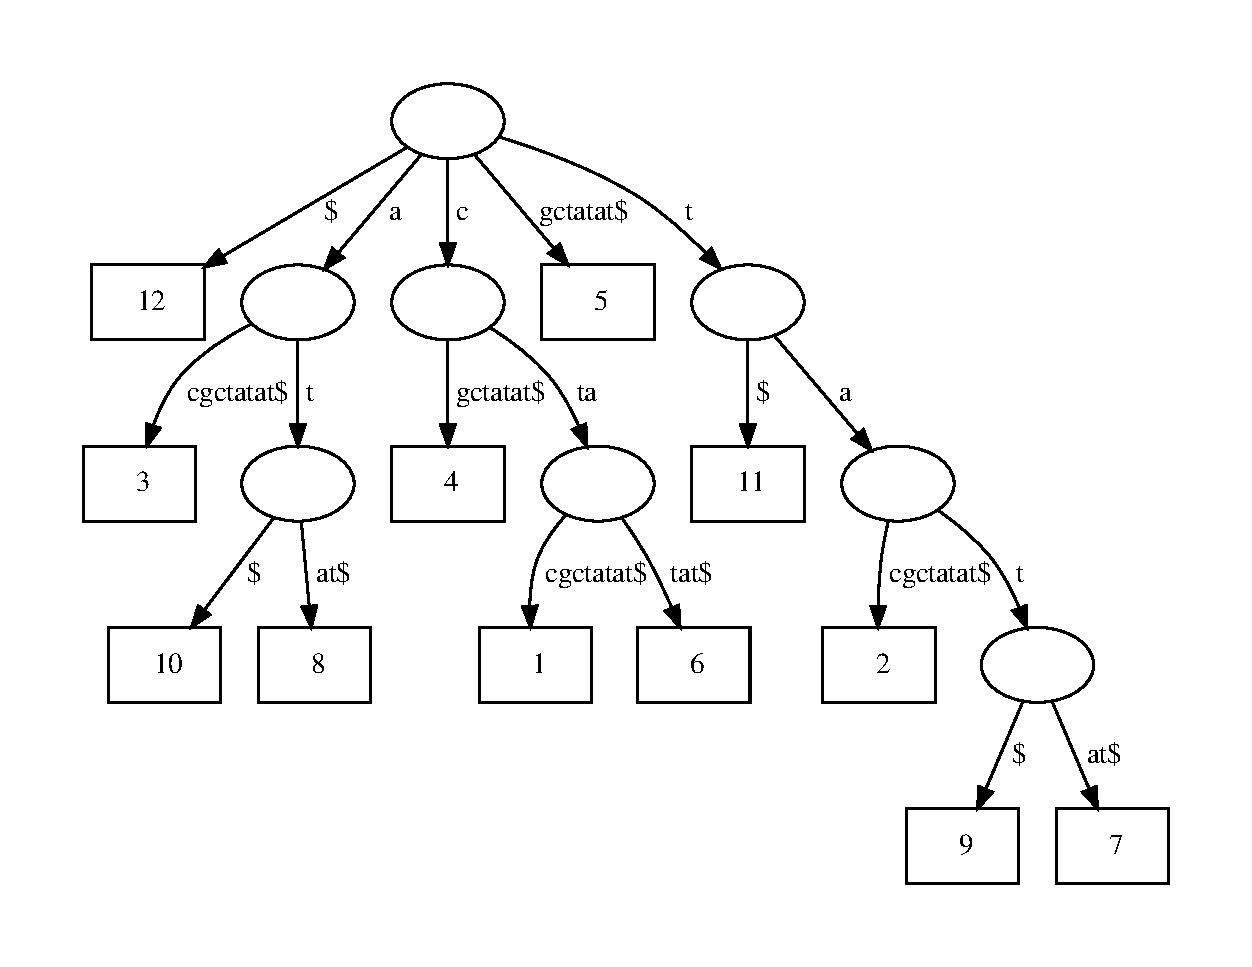
\includegraphics[scale = 0.6]{img/ass3.pdf}
  \end{figure}
  Come detto visualizziamo anche $ST'$, ovvero $ST$ senza foglie e rispettivi
  archi entranti:
  \begin{figure}[H]
    \centering
    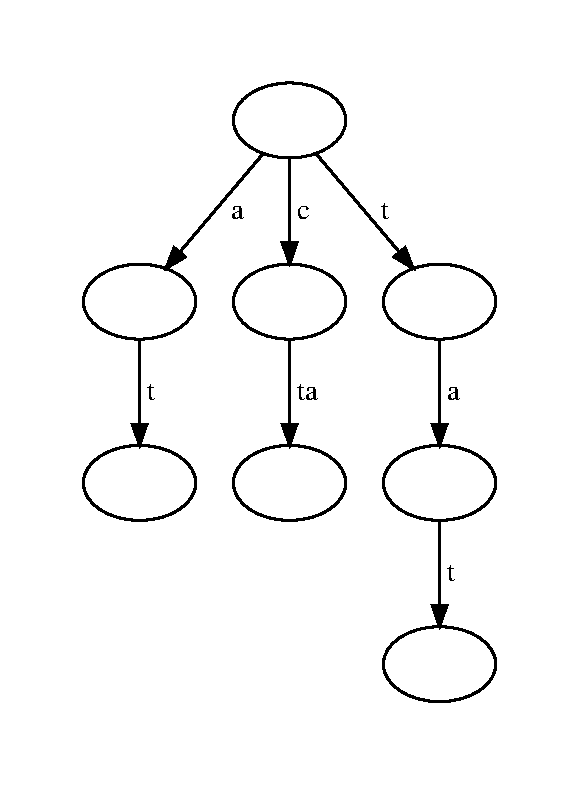
\includegraphics[scale = 0.6]{img/ass3nl.pdf}
  \end{figure}
  \newpage
  Passiamo quindi a studiare la costruzione dell'lcp-intervals tree.\\
  Si ha (con il suffix array inverso riportato per completezza in quanto non
  usato in questo esempio):
  \begin{table}[H]
    \centering
    \begin{tabular}{c|c|c|c|c|}
      & \textbf{SA} & \textbf{SA}$^{-1}$ & \textbf{LCP} & \textbf{suffisso} \\
      \hline
      1 & 12 & 6 & -1 & \$ \\
      2 & 3 & 10 & 0 & acgctatat\$  \\ 
      3 & 10 & 2 & 1 & at\$ \\ 
      4 & 8 & 5 & 2 & atat\$  \\ 
      5 & 4 & 8 & 0 & cgctatat\$  \\ 
      6 & 1 & 7 & 1 & ctacgctatat\$  \\ 
      7 & 6 & 12 & 3 & ctatat\$ \\
      8 & 5 & 4 & 0 & gctatat\$  \\ 
      9 & 11 & 11 & 0 & t\$  \\ 
      10 & 2 & 3 & 1 & tacgctatat\$  \\ 
      11 & 9 & 9 & 2 & tat\$  \\ 
      12 & 7 & 1 & 3 & tatat\$  
    \end{tabular}
  \end{table}
  \noindent
  Procediamo quindi con la costruzione dell'lcp-interval tree.\\
  Si parte dalla radice, rappresentata dall'lcp-interval, con rispettivo valore
  $l$:
  \[0\mbox{-}[1,12]\]
  che è quindi relativo alla stringa vuota $\varepsilon$. Possiamo quindi
  calcolare i relativi $l$-indices, ovvero:
  \[l_0\mbox{-indices}=\{2,5,8,9\}\]
  Possiamo quindi dire che i child sono:
  \[[2,4],[5,7],[8,8],[9,12]\]
  Sappiamo inoltre che gli intervalli di ampiezza 1 non vengono considerati in
  fase di ricostruzione dell'lcp-interval tree in quanto sono facilmente
  individuabile in fase di percorrimento dell'lcp-interval tree anche senza
  averne espclito riferimento in memoria (inoltre si segnala che per questo
  motivo si ottiene una topologia analoga ad un suffix tree privo di foglie). Si
  hanno quindi i seguenti child, per i quali viene indicato anche il loro valore
  $l$, calcolato, dato il rispettivo intervallo $[b,e]$, tramite
  $RMQ(LCP,b+1,e)$: 
  \[1\mbox{-}[2,4],1\mbox{-}[5,7],1\mbox{-}[9,12]\]
  \newpage
  Abbiamo quindi ottenuto i tre child del nodo root, di cui è possibile anche
  indicare $\omega$, come definito precedentemente:
  \begin{itemize}
    \item $1\mbox{-}[2,4]\implies \omega=a$
    \item $1\mbox{-}[5,7]\implies \omega=c$
    \item $1\mbox{-}[9,12]\implies \omega=t$
  \end{itemize}
  Passiamo ad analizzare il primo child, $1\mbox{-}[2,4]$. Calcoliamo i relativi
  $l$-indices, ovvero: 
  \[l_1\mbox{-indices}=\{3\}\]
  Avendo quindi, specificando
  anche il valore $l$ e la relativa $\omega$, solo:
  \[2\mbox{-}[3,4]\implies \omega=at\]
  Essendo l'intervallo di ampiezza due non è necesario proseguire oltre.\\
  Proseguiamo con il secondo child, $1\mbox{-}[5,7]$. Calcoliamo i relativi
  $l$-indices, ovvero: 
  \[l_2\mbox{-indices}=\{6\}\]
  Avendo quindi, specificando
  anche il valore $l$ e la relativa $\omega$, solo:
  \[3\mbox{-}[6,7]\implies \omega=cta\]
  Essendo l'intervallo di ampiezza due, anche in questo caso, non è necesario
  proseguire oltre.\\
  Passiamo infine all'ultimo child, $1\mbox{-}[9,12]$. Calcoliamo i relativi
  $l$-indices, ovvero: 
  \[l_3\mbox{-indices}=\{10\}\]
  Avendo quindi, specificando
  anche il valore $l$ e la relativa $\omega$, solo:
  \[2\mbox{-}[10,12]\implies \omega=ta\]
  In questo caso ho un intervallo di ampiezza tre quindi si prosegue lo studio.
  Calcoliamo gli $l$-indices di $2\mbox{-}[10,12]$, ovvero: 
  \[l_4\mbox{-indices}=\{11\}\]
  Avendo quindi, specificando
  anche il valore $l$ e la relativa $\omega$, solo:
  \[3\mbox{-}[11,12]\implies \omega=tat\]
  Essendo l'intervallo di ampiezza due non è necesario proseguire oltre.\\
  Si segnala, inoltre, come valga quanto detto agli
  lcp-interval embedded, avendo che l'lcp-interval parent "racchiude", anche se
  non strettamente come visto nella definizione teorica, l'lcp-interval child e
  che valga che tutte le $\omega$ dei child contengano come prefisso l'$\omega$
  del rispettivo parent. 
  \newpage
  Si ottiene quindi, nel complesso, la seguente rappresentazione
  dell'lcp-interval tree, a conclusione di quanto detto:
  \begin{figure}[H]
    \centering
    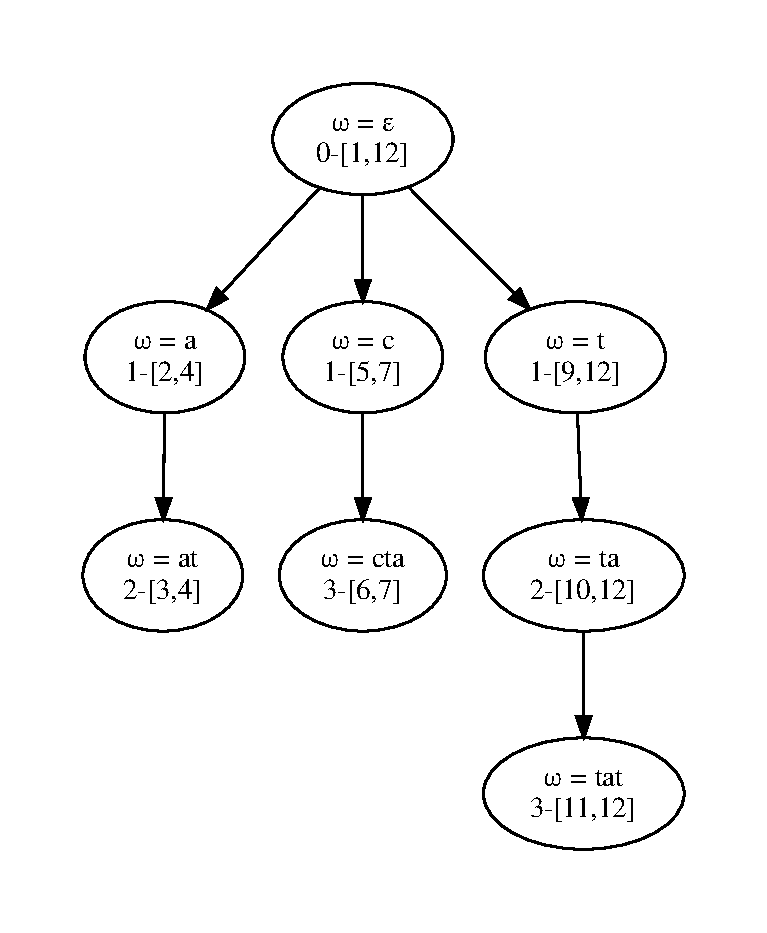
\includegraphics[scale = 0.7]{img/ass3lcp.pdf}
  \end{figure}
  Dando una prova, anche "visuale", di quanto detto anche in merito alla
  relazione tra suffix tree e lcp-interval tree, notando il rapporto tra le path
  label del suffix tree e i $\omega$ dell'lcp-intervals tree, oltre alla
  medesima topologiacondivisa da quest'ultimo e dal suffix tree privo di foglie
  e archi entranti in esse. È interessante anche notare come dai nodi
  dell'lcp-intervals tree, tramite appunto gli lcp-intervals, si possibile
  risalire alla rappresentazione completa del suffix tree tramite il suffix
  array indicato in tabella.\\
  Si prenda ad esempio il nodo, il più profondo nel
  a destra, nell'lcp-intervals tree etichettato con:
  \[\omega =tat\]
  \[3\mbox{-}[11,12]\]
  conferma di quanto detto sul legame tra $\omega$ e path label
  del suffix tree, che in quello stesso nodo arriva, dalla radice, con archi
  etichettati con $t$, $a$ e $t$. \\
  Inoltre, agli indici 11 e 12, abbiamo:
  \[SA[11]=9\mbox{ e }SA[12]=7\]
  che sono gli indici dei suffissi specificati nelle foglie "tagliate" sotto il
  corrispettivo nodo nel suffix tree, ad ulteriore conferma dello stretto
  rapporto tra le due strutture.\\
  Con un ragionamento è possibile ricostruire anche le foglie collegate a nodi
  interni, sfruttando gli intervalli di ampiezza unitaria e i rispettivi valori
  in $SA$, sfruttando eventualmente i "buchi" lasciati dagli intervalli children
  di un nodo, come nel nostro caso per $[8,8]$, che è un "buco" tra $[5,7]$ e
  $[9,12]$ tra i children della radice. Inoltre, qualora si abbia un "buco" di
  ampiezza $k$ maggiore stretta di 1, avendo per costruzione che solo gli
  intervalli di ampiezza 1 non vengono considerati, si può dire di avere $k$
  foglie. Ad esempio immaginiamo di modificare l'esempio visto sopra e ottenere
  come children effettivi della radice nell'lcp-interval tree i seguenti
  intervalli:
  \[1\mbox{-}[2,4],1\mbox{-}[5,6],1\mbox{-}[9,12]\]
  avendo un "buco" tra $[5,6]$ e $[9,12]$ di ampiezza 2. In tal caso potremmo
  dire di avere due foglie, relative gli intervalli $[7,7]$ e $[8,8]$, con i
  relativi indici di suffisso ricavabili dal suffix array.\\ Si
  completa così l'analisi del "mapping" tra le due strutture.
\end{esempio}
\section{Domanda 3}
Si può dimostrare che un algoritmo ottimo elimina fino a due breakpoint ogni
passaggio. Indicando con $b(\pi)$ il numero dei breakpoint presenti
nella permutazione $\pi$ in input, possiamo quindi dire che il numero minimo di
inversioni, $n_{inv}$, necessarie a riordinare $\pi$, ovvero atte a ottenere la
permutazione identica a partire dalla permutazione $\pi$, risponde a:
\[n_{inv}\geq \left\lceil\frac{b(\pi)}{2}\right\rceil\]
Avendo però che ogni step elimina al più due breakpoint (e non, purtroppo,
esattamente due) potrei avere comunque bisogno di più di
$\left\lceil\frac{b(\pi)}{2}\right\rceil$ inversioni, anche se questo è il
limite inferiore sotto al quale sicuramente non si può scendere.\\
La specifica d'uso dell'intero superiore, tramite $\lceil\frac{\,}{\,}\rceil$,
è data dal 
fatto che $\frac{b(\pi)}{2}$, qualora $b(\pi)$ fosse dispari, potrebbe avere
valore decimale. Per quanto detto, avendo l'eliminazione di al più due
breakpoint a inversione, in presenza di un numero dispari di breakpoint, dovrei
aggiungere almeno una singola inversione aggiuntiva, che rappresento nella
disequazione tramite l'intero superiore. Infatti, bisognerebbe fare fare almeno
$\frac{b(\pi)-1}{2}$ inversioni per i primi $b(\pi)-1$ breakpoint, che sono in
numero pari avendo assunto $b(\pi)$ dispari, più l'inversione per il breakpoint
mancante, da cui l'uso dell'intero superiore.   
\subsection{Esempio}
Vediamo quindi un esempio pratico di quanto detto.
\begin{esempio}
  Prendiamo una permutazione $\pi$:
  \[\pi=[\mbox{ 6 1 5 4 3 2 7 }]\]
  Estendiamo $\pi$ con $0$ all'inizio e con
  \[\max_{\pi}+1=7+1=8\]
  alla fine, ottenendo:
  \[\pi=[\mbox{ 0 6 1 5 4 3 2 7 8 }]\]
  Si indicano con `` \textnormal{|}'' i breakpoint:
  \[\pi=[\mbox{ 0 \textnormal{|} 6 \textnormal{|} 1 \textnormal{|}  5 4 3 2
      \textnormal{|} 7 8 }]\] 
  Avendo quindi:
  \[b(\pi)=4\]
  Aspettandoci quindi un minimo numero di inversioni necessarie a
  ottenere la permutazione identica dalla permutazione $\pi$ del tipo:
  \[n_{inv}\geq\left\lceil\frac{4}{2}\right\rceil\geq 2\]
  Si procede quindi con le inversioni.\\
  Effettuiamo in primis l'inversione tra 6 e 1, rispettivamente di indice 1 e 2
  (indicizzando da zero), che rimuove due breakpoint,
  ottenendo, tramite $r(1,2)$:
  \[\pi=[\mbox{ 0 1 \textnormal{|} 6 5 4 3 2
      \textnormal{|} 7 8 }]\]
  Infine si procede con $r(2,6)$, rimuovendo anche i due restanti breakpoint,
  ottenendo la permutazione identica: 
  \[\pi=[\mbox{ 0 1 2 3 4 5 6 7 8 }]\]
  Come si è visto sono state effettuate 2 inversioni, sapendo, per il limite
  inferiore, che non avremmo potuto fare di meglio.\\
  D'altro canto è bene notare
  come sarebbe stato possibile, a differenza dell'esempio mostrato,  avere
  permutazioni, sempre con quattro 
  breakpoint, che avrebbero necessitato di più di due inversioni per ottenere la
  permutazione identica. 
\end{esempio}
\end{document}
% LocalWords:  sottostringhe sottostringa pseudocodice lowercase Hamming
% LocalWords:  sottoalbero sottomatrice sottomatrici pseudocodici
% LocalWords:  algoritmicamente lessicograficamente
